\chapter{Surrogates}
\label{Surrogates}

Although the simulations are quite extensive, it is difficult to apply them directly since they have trouble explaining small adjustments in the control parameters. Especially yawing for the first turbine is limited for 5-degree increments due to the high computational cost of full CDF simulations. In this chapter, we will attempt to train a network which is able to predict behaviour between these known values. Assuming that the network reaches sufficient accuracy, it can then be used to interpolate values for finer adjustments. Like the Weibull model, it is, however, necessary to test the precision of such network before applying it. 


\section{Training data}
\label{trainingdata}

For the training of the network, we will separate the data as $60\%$ training-, $20\%$ validation- and $20\%$ test data. To avoid systematic uncertainties, the data is shuffled before training, so the training, validation, and test are independent between runs. This might, however, lead to an uneven distribution of the configurations in the different sections. Imagine, for example, that every configuration where the pitching is 0 was placed in the test data. This means that we might test on a configuration in which the network is not trained, and the predictions might therefore be very poor. Although it is difficult to ensure this is not the case, when the data is relatively limited, we can check for obvious deficiencies by plotting the distributions when testing. 


\section{Network}

Since the data is limited by the number of simulations, which is relatively small, it makes sense to create a network of similar proportions. To support the claim that such a network is adequate, we will investigate whether additional neurons pose any advantage for lowering the loss function. Since we expect to see the most unpredictable behaviour when the turbulence is highest, we will investigate the closest configuration. Two layers with the same amount of neurons in each allow us to plot the converged loss as a function of neurons per layer. This is done 15 times, and the average loss is calculated for each neuron amount. Additionally, we might assume the loss values to approximately follow a normal distribution, so the standard deviation is computed as a measure for the uncertainty of the average. Plotting the average as a function of the neuron amount, with the standard deviations, yields the graph displayed in figure \ref{fig:neuronloss}

\begin{figure}[H]
    \centering
    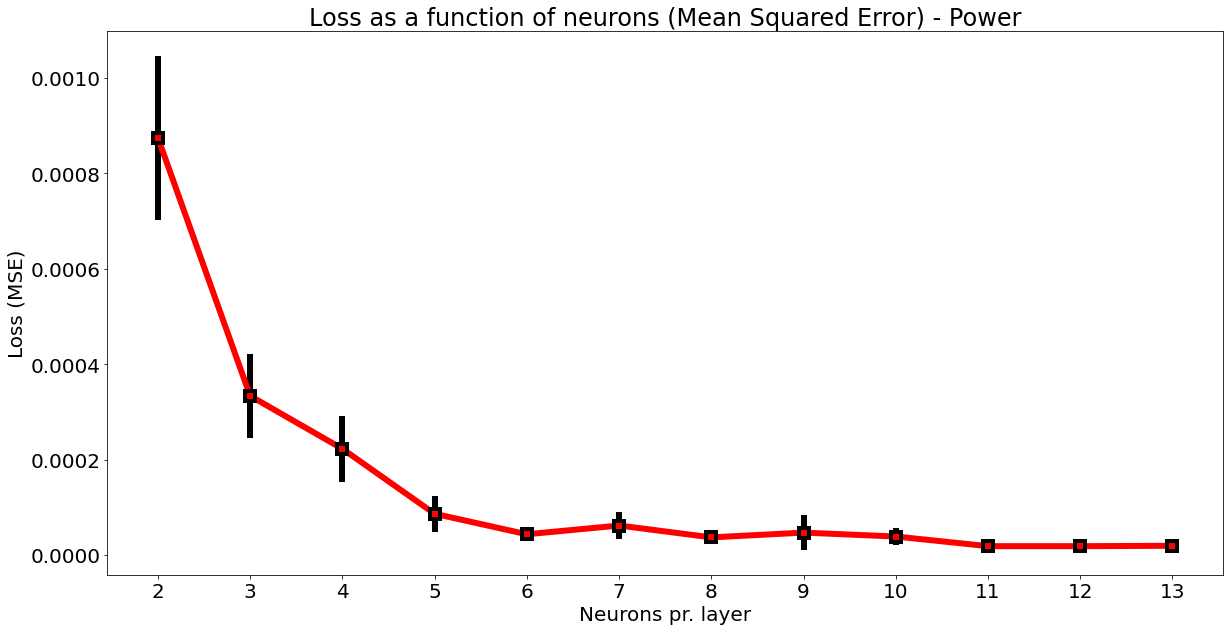
\includegraphics[scale=0.28]{Illustrations/neuron_loss.png}
    \caption{Loss as a function of neuron pr layer}
    \label{fig:neuronloss}
\end{figure}

As we might expect, very low neuron amounts cannot predict the turbine behaviour since it simply does not have enough parameters to describe the correlation. The question then becomes, what is the threshold where more neurons do not pose a clear benefit? What is interesting from figure \ref{fig:neuronloss} is that the graph already seems to flatten out at approximately six neurons. We can also see that the range of uncertainties is large for low numbers of neurons but drastically shrinks as the function converges. The DELs have different dependencies and might therefore require a network of different complexity. For this thesis, however, we will assume this to be sufficient for all cases due to the time constraints of the project. For further analysis, we will use six neurons per layer, as there seems to be no statistical benefit for adding additional complexity. 


\section{Accuracy}

The network has reached a relatively low loss for both training and validation, but this number is difficult to relate to the actual accuracy of the predictions. To get a better intuitive understanding of the validity, we will look at the relative deviation from the predictions to the test data. The purpose is that this data is independent of the training and, therefore, an unbiased verification. Additionally, the loss function is based on scaled values, which is not the case with this approach. The relative deviation can be expressed as the difference between the prediction and the expected value normalized by size. Mathematically it is written as

\begin{equation}
    \delta = \frac{x_a-x_p}{x_a}
\end{equation}

with $x_a$ being the true value and $x_p$ being the prediction. Plotting all the networks, both power, and the different DELs, together as a boxplot yields figure \ref{fig:boxplotacc}

\begin{figure}[H]
    \centering
    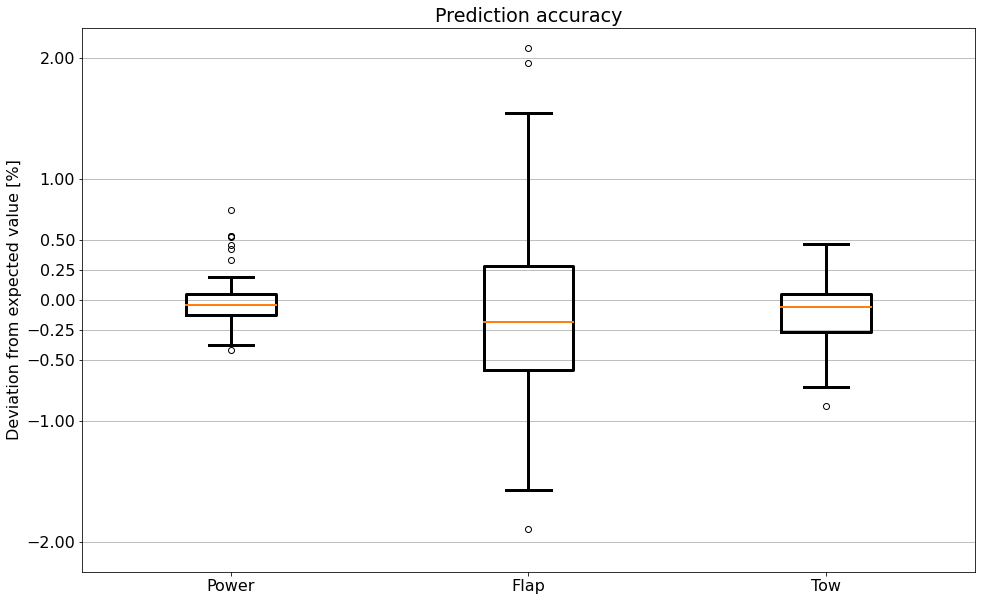
\includegraphics[scale=0.34]{Illustrations/boxplotaccuracy.png}
    \caption{Boxplot of median prediction relative to expected value}
    \label{fig:boxplotacc}
\end{figure}

First, we will note that all measures behave relatively well, with the first and third quantiles nearly within half a percent of the expected outcome. We should also mention that flap load does have some outliers, deviating up to two percent, which is a relatively large deviation compared to the majority of the values but still relatively accurate. We will proceed with this model, though this uncertainty should be considered before making any conclusions. To check for any deficiencies, as mentioned in \ref{trainingdata}, we will plot the control parameter distributions for both training, validation, and test data sets. Doing this yields the histogram displayed in figure \ref{fig:controlparameterdistribution}.

\begin{figure}[H]
    \centering
    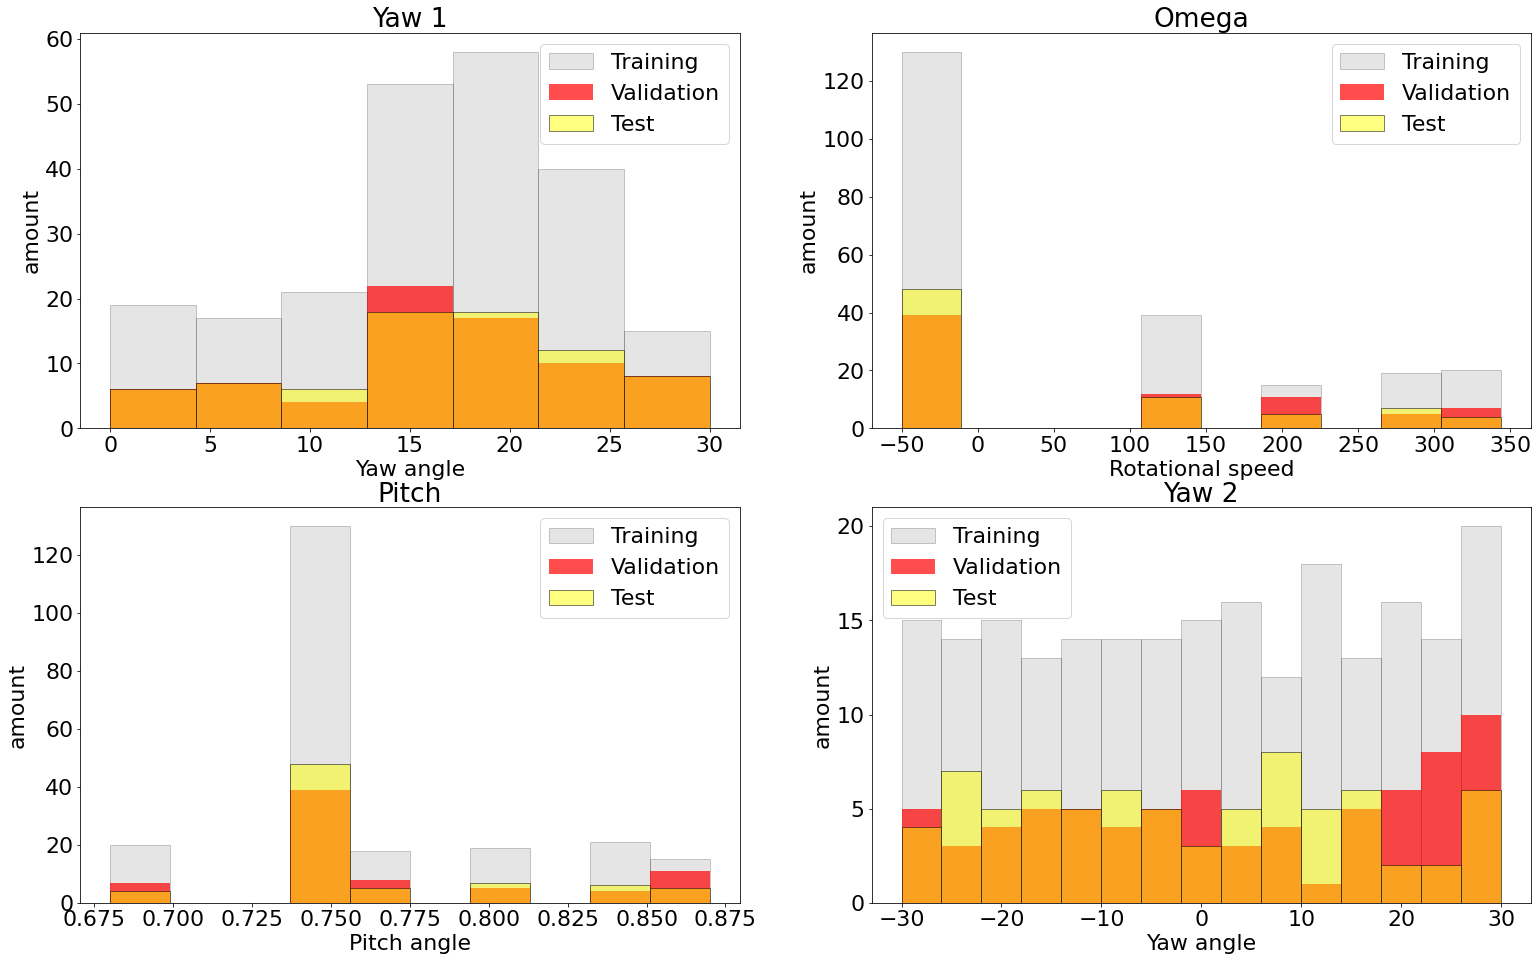
\includegraphics[scale=0.21]{Illustrations/controldistribution.png}
    \caption{Distribution of control parameters}
    \label{fig:controlparameterdistribution}
\end{figure}

Although the data does not seem to be perfectly separated, there are no obvious missing values either. We must therefore conclude that the performance of the model cannot be explained by the data separation and might instead be caused by the unpredictable nature of the moments. As future work, it might make sense to investigate whether more complex networks could explain this behaviour more consistently,

To give a practical example of how the whole process works, we will plot the Weibull prediction with the data, similar to what we did in figure \ref{fig:weibullexample}. Again taking the power distribution for an arbitrary configuration from the test data, gives us the graph displayed in figure \ref{fig:predictweibull}

\begin{figure}[H]
    \centering
    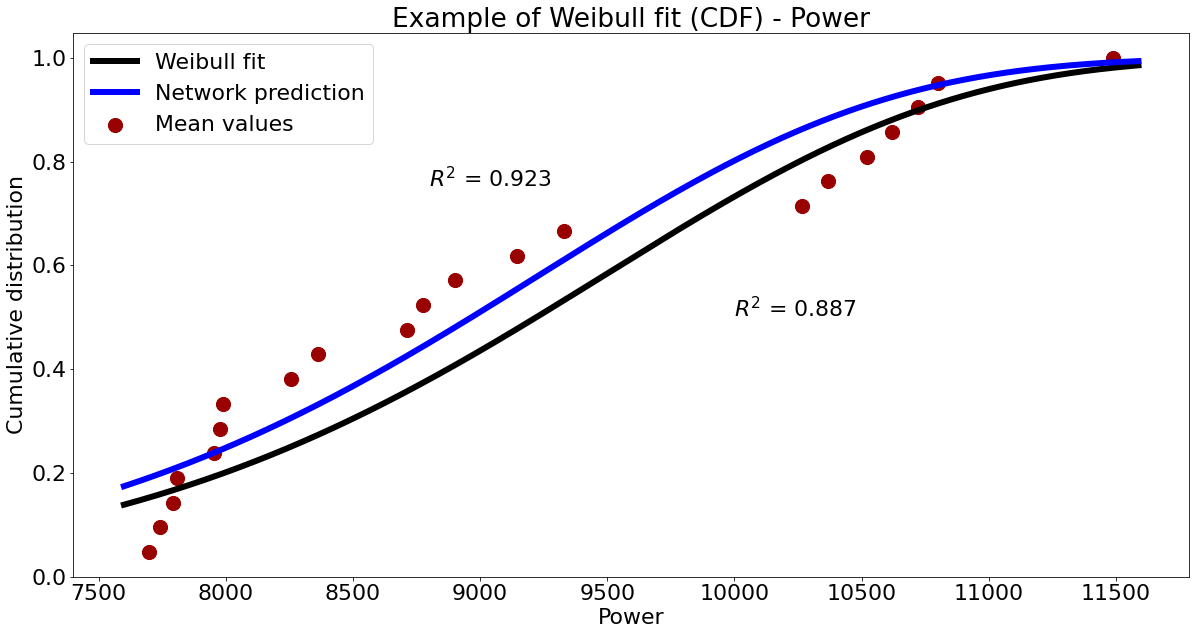
\includegraphics[scale=0.25]{Illustrations/predictiontestplot.png}
    \caption{Network prediction for $\psi_1 = 25^\circ, \; \theta_1 = -0.5^\circ, \; \Omega_1 = 0.75 \frac{m}{s}, \; \psi_2 = 15^\circ$}
    \label{fig:predictweibull}
\end{figure}

Here we see quite an interesting outcome, as the predicted curve actually explains the variance better than the original fit. Although this might seem impossible at first glance, the fit is behaving as expected. The mysterious behaviour should instead be explained as a limitation of the evaluation method, for which we chose to apply the coefficient of determination. The fit, applied through Scipy \cite{scipy}, is, as previously mentioned, determined by maximum likelihood estimation \cite{maxlikelihood} and is therefore not meant to find the lowest possible $R^2$. Although it is out of the scope of this project to explain exactly how this works, it is important to note why this deviation occurs. Intuitively it should be clear that the prediction follows the data, and the $R^2$-value support this suspicion being over 0.92, which statistically proves a strong correlation. Ultimately this proves that the methodology, although not perfect, is good enough for the purpose, and we can proceed to the optimization.  